% Figure 2, top (fig:rank-selector): the RankSelect circuit as a chain of N
% per-position cells.  The tikzpicture is verbatim from main.tex in
% ~/src/qcaai/qce26/paper; the Makefile renders it to an SVG of paths.
\documentclass[dvisvgm]{standalone}
\usepackage{amsmath,amssymb}
\usepackage{tikz}
\begin{document}
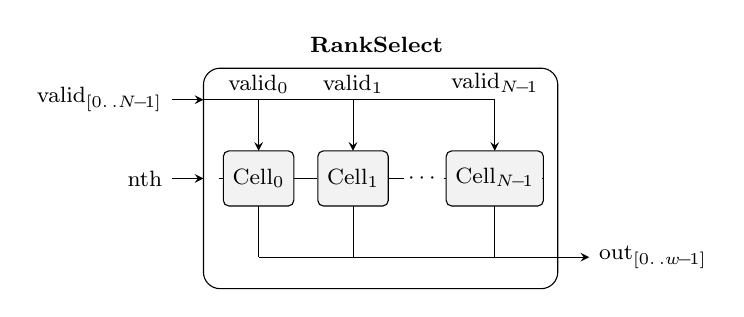
\begin{tikzpicture}[
  cell/.style={draw, fill=gray!10, minimum width=0.7cm, minimum height=0.7cm,
               rounded corners=2pt, font=\footnotesize},
  lbl/.style={font=\footnotesize},
  arr/.style={->, >=stealth},
]
  % Cells
  \node[cell] (c0) at (0,0) {Cell$_0$};
  \node[cell] (c1) at (1.2,0) {Cell$_1$};
  \node[lbl]  (dots) at (2.1,0) {$\cdots$};
  \node[cell] (cn) at (3.0,0) {Cell$_{N\!-\!1}$};

  % Threading wire: nth through cells
  \draw (-0.5, 0) -- (c0.west);
  \draw (c0.east) -- (c1.west);
  \draw (c1.east) -- (1.85, 0);
  \draw (2.35, 0) -- (cn.west);
  \draw (cn.east) -- (3.6, 0);

  % Per-cell inputs from top (v_i fan-out)
  \foreach \x/\lab in {0/$v_0$, 1.2/$v_1$, 3.0/$v_{N\!-\!1}$} {
    \draw[arr] (\x, 1.0) -- (\x, 0.35);
  }
  \node[lbl] at (0, 1.2) {$\text{valid}_0$};
  \node[lbl] at (1.2, 1.2) {$\text{valid}_1$};
  \node[lbl] at (3.0, 1.2) {$\text{valid}_{N\!-\!1}$};

  % Per-cell outputs drop to gather bus (no arrowheads)
  \foreach \x in {0, 1.2, 3.0} {
    \draw (\x, -0.35) -- (\x, -1.0);
  }

  % Encapsulating RankSelect box
  \draw[rounded corners=6pt] (-0.7,-1.4) rectangle (3.8,1.4);
  \node[font=\footnotesize\bfseries] at (1.5,1.7) {RankSelect};

  % - External inputs on the left -
  % v[0..N-1]: short arrow into left side, then fan-out line across top
  \draw[arr] (-1.1, 1.0) -- (-0.7, 1.0);
  \node[lbl, left] at (-1.1, 1.0) {$\text{valid}_{[0\mathinner{.\,.}N\!-\!1]}$};
  % horizontal fan-out bus along top inside box
  \draw (-0.7, 1.0) -- (3.0, 1.0);

  % nth: short arrow into left side at the threading wire level
  \draw[arr] (-1.1, 0) -- (-0.7, 0);
  \node[lbl, left] at (-1.1, 0) {nth};

  % - External output on the right -
  % shared w-qubit output bus along bottom, then short arrow out right
  \draw (0, -1.0) -- (3.8, -1.0);
  \draw[arr] (3.8, -1.0) -- (4.2, -1.0);
  \node[lbl, right] at (4.2, -1.0) {$\text{out}_{[0\mathinner{.\,.}w\!-\!1]}$};
\end{tikzpicture}
\end{document}
